\documentclass[tikz,border=10pt]{standalone}
\usepackage{amsmath}
\usetikzlibrary{arrows.meta,calc,decorations.pathreplacing}

\begin{document}
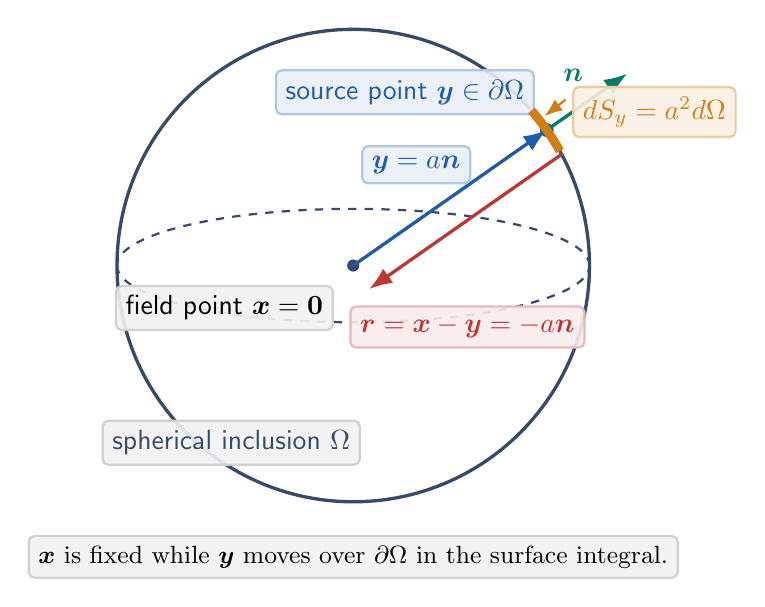
\begin{tikzpicture}[
  >=Latex,
  font=\sffamily,
  thick,
  textbox/.style={rounded corners=2pt,inner sep=3.5pt,fill opacity=0.90,text opacity=1},
  sourcebox/.style={textbox,fill=source!10,draw=source!35},
  relativebox/.style={textbox,fill=relvec!10,draw=relvec!35},
  surfacebox/.style={textbox,fill=surface!12,draw=surface!40},
  neutralbox/.style={textbox,fill=black!5,draw=black!18}
]
\definecolor{boundary}{RGB}{55,75,105}
\definecolor{source}{RGB}{32,92,170}
\definecolor{normal}{RGB}{0,125,105}
\definecolor{relvec}{RGB}{190,55,55}
\definecolor{surface}{RGB}{210,125,20}

\coordinate (O) at (0,0);
\coordinate (Y) at ({3.0*cos(35)},{3.0*sin(35)});
\coordinate (N) at ({4.25*cos(35)},{4.25*sin(35)});

% Spherical inclusion shown by a meridional circle and a dashed equator.
\draw[boundary,very thick] (O) circle (3.0);
\draw[boundary,dashed] (-3,0) arc[start angle=180,end angle=360,x radius=3,y radius=0.72];
\draw[boundary,dashed] (3,0) arc[start angle=0,end angle=180,x radius=3,y radius=0.72];
\node[boundary,neutralbox] at (-1.55,-2.25) {spherical inclusion $\Omega$};

% Field point at the centre.
\fill[boundary] (O) circle (2.2pt);
\node[neutralbox,below left=7pt] at (O)
  {field point $\boldsymbol x=\boldsymbol0$};

% Source point and radius vector.
\fill[source] (Y) circle (2.5pt);
\draw[->,source,very thick] (O)--(Y);
\node[source,sourcebox] at (0.80,1.28) {$\boldsymbol y=a\boldsymbol n$};
\node[source,sourcebox,anchor=east] at ($(Y)+(-0.15,0.48)$)
  {source point $\boldsymbol y\in\partial\Omega$};

% Outward normal.
\draw[->,normal,very thick] (Y)--(N)
  node[pos=0.62,above left=1pt] {$\boldsymbol n$};

% Relative vector from source to field point, offset slightly for readability.
\draw[->,relvec,very thick]
  ($(Y)+(0.20,-0.30)$)--($(O)+(0.20,-0.30)$);
\node[relvec,relativebox] at (1.45,-0.78)
  {$\boldsymbol r=\boldsymbol x-\boldsymbol y=-a\boldsymbol n$};

% Small surface element near the source point.
\draw[surface,line width=3.2pt]
  ({3*cos(29)},{3*sin(29)}) arc[start angle=29,end angle=41,radius=3];
\draw[surface,->] ({3.42*cos(38)},{3.42*sin(38)})--({3.08*cos(38)},{3.08*sin(38)});
\node[surface,surfacebox,anchor=west] at (2.78,1.95) {$dS_y=a^2d\Omega$};

\node[neutralbox,align=center,font=\small] at (0,-3.70)
  {$\boldsymbol x$ is fixed while $\boldsymbol y$ moves over $\partial\Omega$ in the surface integral.};
\end{tikzpicture}
\end{document}
